\documentclass[output=paper,colorlinks,citecolor=brown]{langscibook}

\title{On the Ngbugu vowel system}

\hyphenation{Ngbugu}
\hyphenation{RefLex}

\author{Kenneth S. Olson\affiliation{SIL International}
}

\abstract{Previous researchers have posited asymmetric \is{symmetry} oral \isi{vowel systems} for \ili{Ngbugu} and other \ili{Banda languages}. The present analysis shows that \ili{Ngbugu} has a symmetric 10-vowel system which includes one interior vowel \is{interior vowels} /ə/ and lacks \isi{vowel harmony}. It also supports and refines \citegen{BoyeldieuCloarec-Heiss2001} proposed \ili{Proto-Banda} vowel system. The affinities of the resulting proto vowel system to those of nearby languages could facilitate the comparison of vowel systems across the region in order to test hypotheses about \isi{shared inheritance} or \isi{borrowing}. Possible explanations for the lack of \isi{vowel harmony} are suggested.
}

\IfFileExists{../localcommands.tex}{%hack to check whether this is being compiled as part of a collection or standalone
  \addbibresource{localbibliography.bib}
  \usepackage{langsci-optional,langsci-branding}
\usepackage{langsci-gb4e}
% \usepackage{langsci-textipa}
% \usepackage{langsci-glyphs}
\usepackage[linguistics]{forest}
\usepackage{tabto}
\usepackage{multirow}
\usepackage{bbding}

\usepackage[normalem]{ulem}

\usepackage{tikz-qtree}

\usepackage{enumitem}

\usepackage{multicol}
\usepackage{stmaryrd} %double brackets

\makeatletter
\let\pgfmathModX=\pgfmathMod@
\usepackage{pgfplots,pgfplotstable}%
\let\pgfmathMod@=\pgfmathModX
\makeatother
\usepgfplotslibrary{colorbrewer}
\usetikzlibrary{fit}

\usepackage{jambox}
\usepackage{tikz-qtree-compat}
\usetikzlibrary{arrows, arrows.meta}
\usepackage{longtable}
\usepackage{subcaption}

  \makeatletter
\let\thetitle\@title
\let\theauthor\@author
\makeatother

\newcommand{\togglepaper}[1][0]{
%   \bibliography{../localbibliography}
  \papernote{\scriptsize\normalfont
    \theauthor.
    \thetitle.
    To appear in:
    Change Volume Editor \& in localcommands.tex
    Change volume title in localcommands.tex
    Berlin: Language Science Press. [preliminary page numbering]
  }
  \pagenumbering{roman}
  \setcounter{chapter}{#1}
  \addtocounter{chapter}{-1}
}

\newcommand{\bari}{\ipabar{\i}{.5ex}{1.1}{}{}}
\newcommand{\notipa}[1]{\textnormal{#1}}

\newcommand{\agre}{\textsc{agr}-\ol{eene}}

\renewcommand{\emph}[1]{\textit{#1}} % resetting a setting from ling-macros-modified (I think?)

% forest settings to make compact but (mostly) straight-spined trees:
\forestset{
fairly nice empty nodes/.style={
            delay={where content={}{shape=coordinate,for parent={
                  for children={anchor=north}}}{}}
, angled/.style={content/.expanded={$<$\forestov{content}$>$}}
}}

\forestset{sn edges/.style={for tree={parent anchor=south, child anchor=north}}}

\newcommand{\bex}{\begin{exe}}
\newcommand{\fex}{\end{exe}}

\newcommand{\bxl}{\begin{exe}}
\newcommand{\fxl}{\end{exe}}

\newcommand{\ix}[1]{\textsubscript{#1}}
\newcommand{\alert}[1]{\textbf{#1}}
\newcommand{\ol}[1]{\textit{#1}}


			\usetikzlibrary{shapes,arrows,positioning,decorations,decorations.pathmorphing,intersections}
\forestset{
nice empty nodes/.style={
    for tree={calign=fixed edge angles},
    delay={where content={}{shape=coordinate,for siblings={anchor=north}}{}}
},
}

\definecolor{dark-gray}{gray}{0.3}

%\usepackage{dingbat,pifont}


%%%%%%%%%%%%For arrows%%%%%%%%%%%%%

\newcommand\Tikzmark[2]{%
  \tikz[remember picture]\node[inner sep=0pt,outer sep=0pt] (#1) {#2};%
}
\NewDocumentCommand\DrawArrow{O{}mmmmO{3}}{
\tikz[remember picture,overlay]
  \draw[->,line width=0.8pt,shorten >= 2pt,shorten <= 2pt,#1]
    (#2) -- ++(0,-#6\ht\strutbox) coordinate (aux) -- node[#4] {#5} (#3|-aux) -- (#3);
}
\NewDocumentCommand\DrawDotted{O{}mmmmO{3}}{
\tikz[remember picture,overlay]
  \draw[->,line width=0.9pt,dotted,shorten >= 2pt,shorten <= 2pt,#1]
    (#2) -- ++(0,-#6\ht\strutbox) coordinate (aux) -- node[#4] {#5} (#3|-aux) -- (#3);
}
\NewDocumentCommand\DrawLine{O{}mmmmO{3}}{
\tikz[remember picture,overlay]
  \draw[line width=0.8pt,shorten >= 2pt,shorten <= 2pt,#1]
    (#2) -- ++(0,-#6\ht\strutbox) coordinate (aux) -- node[#4] {#5} (#3|-aux) -- (#3);
}
%%%%%%%%%%%%%%%%%%%%%%%%%%%%%%%%%%%%%


\newcommand{\baru}{ʉ}
\newcommand{\baruH}{\'\baru}
\newcommand{\baruL}{\`\baru}

\newcommand{\ep}{ε}
\newcommand{\epH}{\'\ep}
\newcommand{\epL}{\`\ep}

\newcommand{\schwa}{ə}
\newcommand{\schwaH}{\'ə}
\newcommand{\schwaL}{\`ə}

\newcommand{\oo}{ɔ}
\newcommand{\ooH}{\'\oo}
\newcommand{\ooL}{\`\oo}

\newcommand{\ds}{\textsuperscript{
	\hspace*{-2pt}\begin{tikzpicture}
		\draw[-{>[scale=0.5]}] (0,0.4) --(0,0.25);
	\end{tikzpicture}}}

\newcommand{\ch}{t͡ʃ}
\newcommand{\dz}{d͡ʒ}

\newcommand{\tgl}{ʔ}

%shortcuts for the complementizers
\newcommand{\mbuL}{mb\baruL}
\newcommand{\mbuHL}{mb\baruH\baruL}
\newcommand{\mbuLH}{mb\baruL\baruH}
\newcommand{\la}{lá}
\newcommand{\nda}{ndà}

\newcommand{\tsc}[1]{\textsc{#1}}
\renewcommand{\textscb}{ʙ}
\newcommand{\ipa}[1]{#1} %disable IPA

\newcommand{\SM}[1]{#1}

\DeclareNewSectionCommand
  [
    counterwithin = chapter,
    afterskip = 2.3ex plus .2ex,
    beforeskip = -3.5ex plus -1ex minus -.2ex,
    indent = 0pt,
    font = \usekomafont{section},
    level = 1,
    tocindent = 1.5em,
    toclevel = 1,
    tocnumwidth = 2.3em,
    tocstyle = section,
    style = section
  ]
  {appendixsection}

\renewcommand*\theappendixsection{\Alph{appendixsection}}
\renewcommand*{\appendixsectionformat}
              {\appendixname~\theappendixsection\autodot\enskip}
\renewcommand*{\appendixsectionmarkformat}
              {\appendixname~\theappendixsection\autodot\enskip}

\renewcommand{\lsChapterFooterSize}{\footnotesize}

\togglepaper[23]
}{}


\begin{document}
\maketitle

\section{Introduction}\label{sec:olson:1}

Authors of previous studies have proposed various oral \isi{vowel systems} for \ili{Ngbugu} (ISO 639-3 code=lnl), a language of the Banda \il{Banda languages} group, Ubangian \il{Ubangian languages} family, spoken in southcentral \isi{Central African Republic} by about 95,000 people \citep{SimonsFennig2018}. These proposed systems are shown in Tables \ref{tab:olson:1}, \ref{tab:olson:2}, and \ref{tab:olson:3}.\footnote{I use standard IPA transcriptions for segments and tone in this paper.}

\begin{table}
\caption{\ili{Ngbugu} oral vowels \citep[13--14]{Cloarec-Heiss1978}}
\label{tab:olson:1}
    \begin{tabular}{llll}
    \lsptoprule
                & front & central & back\\
    \midrule
        high    & i     & ɨ       & u\\
        mid     & e     & ə       & o\\
        low     &       & a       & ɔ\\
    \lspbottomrule
    \end{tabular}
\end{table}

The system in \tabref{tab:olson:1} contradicts a universal \is{language universals} put forth by \citet[122]{Crothers1978}: “The number of height \is{vowel height} distinctions in front vowels is equal to or greater than the number in back vowels.” Yet, the majority of \ili{Banda languages} appear to exhibit it. \citet[13--16]{Cloarec-Heiss1978} posits this same system for seven other Banda \il{Banda languages} speech varieties: \ili{Langbasi} [lna], \ili{Ngundu} [nue], \ili{Kpagua} [kuw], \ili{Gubu} [gox], \ili{Gbi} [bbp], \ili{Linda} [liy], and \ili{Yakpa} [bjo]. It is also the system posited for \ili{Mono} [mnh] by both \citet{Kamanda-Kola2003} and \citet{Olson2005} independently of each other.

\begin{table}
\caption{\ili{Ngbugu} oral vowels \citep[43]{Théret-Kieschke1998}}
\label{tab:olson:2}
    \begin{tabular}{llll}
    \lsptoprule
                    & front & central & back\\
    \midrule
        high        & i     & ɨ       & u\\
        mid         & e     & ə       & o\\
        low         & ɛ     & a       & (ɔ)\\
        diphthongs  & iɛ    &         & oa\\
    \lspbottomrule
    \end{tabular}
\end{table}

\citeauthor{Théret-Kieschke1998}’s proposed system in \tabref{tab:olson:2} is more \is{symmetry} symmetric. In addition to monophthongs, she posits two \isi{diphthongs}. She considers /ɔ/ to be a marginal phoneme \is{marginal phonemes} (p. 9).

\begin{table}
\caption{\ili{Ngbugu} oral vowels \citep[191]{BoyeldieuCloarec-Heiss2001}}
\label{tab:olson:3}
    \begin{tabular}{llll}
    \lsptoprule
                & front & central & back\\
    \midrule
    high        & i     & ɨ       & u\\
    mid         & e     & ə       & ɔ\\
    low         & (i)ɛ  & a       &\\
    \lspbottomrule
    \end{tabular}
\end{table}

\citeauthor{BoyeldieuCloarec-Heiss2001} propose the system shown in \tabref{tab:olson:3}. They transcribe the low front vowel as /(i)ɛ/, capturing the generalization -- according to their data -- that the phoneme is usually realized as [iɛ], yet surfaces as [ɛ] in initial position and immediately following /w/. The vowel /ɔ/ is positioned as a mid vowel in their chart, along with /e/ and /ə/ (p. 192).\footnote{Boyeldieu (pers. comm.) considers /ɔ/ to be phonetically halfway between [o] and [ɔ] when it does not follow a /w/.}

Comparison of these three proposed systems \is{vowel systems} raises questions about the phonemic status of /ɛ/, /o/, and /ɔ/. To address these questions, I worked with a team of three native \ili{Ngbugu} speakers during three visits to Bangui from 2015 to 2017 (a total of five weeks) to re-evaluate the oral vowel system, employing the \isi{participatory research} methodology elucidated in \citet{Kutsch-Lojenga1996}.\footnote{The three language consultants conducted extensive orthography testing in the \ili{Ngbugu} region during this period of time.}  I do not address \isi{diphthongs} or \isi{nasal vowels}, which are both also part of the \ili{Ngbugu} \is{vowel systems} vowel system.

Prior to our consultations, the team had collected a corpus of about 2000 lexical items. We removed compound words, borrowings, derived words, etc., after which we had a corpus of about 700 words to work with.

In \sectref{sec:olson:2}, I provide evidence for the phonemic status of /ɛ/, /o/, and /ɔ/, as well as an in-progress \isi{merger} between /o/ and /ɔ/. I also provide evidence for the existence of an additional vowel /ʊ/ not reported by the previous researchers. In \sectref{sec:olson:3}, I provide acoustic evidence for my transcription of the vowels and show that /ɨ/ is best reinterpreted as the front vowel /ɪ/. In \sectref{sec:olson:4}, I discuss possible implications for the historical development of vowels in the Banda \il{Banda languages} group.

\section{Phonology}\label{sec:olson:2}

Several arguments support the phonemic status of /ɛ/. First, contrasts between /ɛ/ and its phonetically similar segment /e/ are common in \ili{Ngbugu}. A sampling of these contrasts is shown in \tabref{tab:olson:4}.

\begin{table}
\caption{Contrasts between /ɛ/ and /e/}
\label{tab:olson:4}
    \begin{tabular}{l l l l}
    \lsptoprule
        /ɛ/ & gloss & /e/  & gloss\\
    \midrule
        ʃé.ʃɛ̄ & bifurcation & ʃē.ʃē & root\\
        ɲɛ́  & all, together  & ɲé    & \textsc{2pl}-object\\
        ɛ̄     & small       & ʔē    & call\\
        húɛ̄   & sweat       & hùè   & open\\
    \lspbottomrule
    \end{tabular}
\end{table}

Second, my language consultants had no difficulty distinguishing /ɛ/ and /e/, and the orthography testing they conducted in the \ili{Ngbugu} community suggested that this is true among \ili{Ngbugu} speakers in general. Third, /ɛ/ is not rare, occurring in more than 20 words in our corpus. This count does not include word-initial [ɛ̄], which may be a relic of an historical prefix denoting animals \citep[13]{Greenberg1970}. Fourth, /ɛ/ occurs in word-initial, word-medial, and word-final positions, as shown in \tabref{tab:olson:5}.

\begin{table}
\caption{Distribution of /ɛ/}
\label{tab:olson:5}
    \begin{tabular}{lll}
    \lsptoprule
                    & /ɛ/ & gloss\\
    \midrule
        initial     & ɛ̄.vʁó & dog\\
        medial      & ŋɡʊ́.lɛ̀.ʃò  & earthworm\\
        final       & ʃé.ʃɛ̄   & bifurcation\\
    \lspbottomrule
 \end{tabular}
\end{table}

While the phonetic sequence [iɛ] does occur in a substantial number of words, it is also true that [ɛ] is attested immediately following more consonants than just /w/, e.g. [ŋɡʊ́.lɛ̀.ʃò] ‘earthworm’, [ʃé.ʃɛ̄] ‘bifurcation’, [ɡbɛ́] ‘all’, [ndɛ̀.rə̀] ‘sticky’. Additional examples are found in Boyeldieu's \ili{Ngbugu} wordlist in \textit{RefLex} \citep{SegererFlavier2011}. There are also cases where [iɛ] and [ɛ] both occur after the same consonant, e.g. [ɡbīɛ̄] ‘king’ vs. [ɡbɛ́] ‘all’. These considerations bolster the view that /ɛ/ is a phoneme in its own right, distinct from the diphthong /iɛ/.

Finally, there is a clear acoustic distinction between /ɛ/ and /e/, as discussed below in \sectref{sec:olson:3}.

Several arguments support the phonemic status of both /o/ and /ɔ/. First, there is contrast between these two phonetically similar segments, as shown in \tabref{tab:olson:6}.

\begin{table}
\caption{Contrasts between /o/ and /ɔ/}
\label{tab:olson:6}
    \begin{tabular}{llll}
    \lsptoprule
        /o/ & gloss & /ɔ/  & gloss\\
    \midrule
        kpò.tò & hat & kpɔ̀.tɔ̀ & skin\\
        ko  & (to) distribute  & kɔ & (to) oil \citep[9]{Théret-Kieschke1998}\\
    \lspbottomrule
    \end{tabular}
\end{table}

Second, many native speakers have no difficulty distinguishing the two sounds. Third, both sounds are common, each occurring in more than 30 words in my corpus. Fourth, there is a clear acoustic distinction between the two sounds, as discussed below in \sectref{sec:olson:3}.

Despite this evidence, the case of /o/ and /ɔ/ is complicated by a couple of factors. First, for apparently all speakers of \ili{Ngbugu} -- even those for whom the two sounds are contrastive -- \isi{free variation} occurs between /o/ and /ɔ/ for certain lexical items, as exemplified in \tabref{tab:olson:7}.

\begin{table}
\caption{Free variation between /o/ and /ɔ/ in some lexical items}
\label{tab:olson:7}
    \begin{tabular}{ll}
    \lsptoprule
        /o/ \char`\~ \space /ɔ/ & gloss\\
    \midrule
        kò.tò \char`\~ \space kɔ̀.tɔ̀ & hill\\
        kò.kò.lò \char`\~ \space kɔ̀.kɔ̀.lɔ̀  & duck\\
    \lspbottomrule
    \end{tabular}
\end{table}

Second, while all three of my language consultants recognize the distinctiveness of /o/ and /ɔ/, they indicate that some \ili{Ngbugu} speakers do not distinguish the two sounds, opting to produce /o/ in all cases. \citet[9]{Théret-Kieschke1998} noted this pattern among younger speakers and suggested that a \isi{merger} is currently underway between /o/ and /ɔ/: *o, *ɔ > o. Robust contrast exists between /o/ and /ɔ/ in most other Banda \il{Banda languages} varieties, e.g. \ili{Linda} \citep{BoyeldieuCloarec-Heiss2001} and \ili{Mono} \citep{Olson2005}, which harmonizes well with this claim.

During the course of our research, we encountered an additional synchronic vowel phoneme, /ʊ/, not attested by previous researchers. Several factors support the existence of this additional phoneme. First, there is contrast between /ʊ/ and all of the other back vowels, as shown in \tabref{tab:olson:8}.

\begin{table}
\caption{Contrast between /ʊ/ and other back vowels}
\label{tab:olson:8}
    \begin{tabular}{llllllll}
    \lsptoprule
        /u/     & gloss & /ʊ/ & gloss & /o/ & gloss & /ɔ/ & gloss\\
    \midrule
        kū      & thigh & kʊ̄ & war & kō & male & kɔ̀ & type of termite\\
        --     & & ʁʊ̀ & stroll & ʁò & roll, pass & -- & \\
        tū      & ear & tʊ̀.ʁʊ̀ & in vain & dò & divert & tɔ̀ & marry\\
        --     & & ɡʁʊ̄ & hole & ɡʁó & white & -- & \\
    \lspbottomrule
    \end{tabular}
\end{table}

Second, native speakers readily distinguish /ʊ/ from other back vowels. Third, /ʊ/ is not rare, occurring in over 40 lexical items in my corpus. Fourth, /ʊ/ occurs both medially and finally, e.g. [sʊ̀.ɡʊ́] ‘pillar’. Finally, /ʊ/ is distinct acoustically from the other back vowels, as discussed in \sectref{sec:olson:3}.

While /ʊ/ does not occur as such in any of the previous research, it does show up indirectly in \citet{BoyeldieuCloarec-Heiss2001}, where the sequence transcribed there as /wɔ/ corresponds to my /ʊ/, as shown in \tabref{tab:olson:9}.\footnote{Most of the occurrences of [ʊ] in \tabref{tab:olson:9} occur after [ʁ], but most cases of [ʊ] in my corpus follow other consonants. The difference between my data and that of Boyeldieu and Cloarec-Heiss could be due in part to dialectal variation. More research is necessary on this.}

\begin{table}
\caption{Samples of /ʊ/ transcribed as /wɔ/ by \citet{BoyeldieuCloarec-Heiss2001}}
\label{tab:olson:9}
    \begin{tabular}{llll}
    \lsptoprule
        Boyeldieu and Cloarec-Heiss & page & my transcription & gloss\\
    \midrule
        jɔ̄ʁwɔ̀ & 216 & dʒō.ʁʊ̀ & sorghum\\
        gʁwɔ & 218 & ɡʁʊ̀ & to touch\\
        gwɔ̀gwɔ̀ & 218 & ɡʊ̀ & hunger\\
        kʁwɔ & 218 & kʁʊ̀ & to stop\\
        ngʁwɔ & 195, 218 & ŋɡʁʊ̀ & to scratch\\
        ʁwɔ & 213 & ʁʊ̀ & to walk\\
        tɔ̀ʁwɔ̀ & 212 & tʊ̀.ʁʊ̀ & in vain\\
    \lspbottomrule
    \end{tabular}
\end{table}

Though \citeauthor{BoyeldieuCloarec-Heiss2001} do not document extant /ʊ/ per se, their comparative study of \ili{Ngbugu} and \ili{Linda} leads them to reconstruct the high back [–ATR] vowel *ʊ for \ili{Proto-Banda} (pp. 199, 202--203). One of the key findings of the current paper is that the reflex /ʊ/ of the proto phoneme *ʊ is present in \ili{Ngbugu} today.

This finding suggests a possible novel use of the \isi{comparative method} -- as an aid to \isi{linguistic fieldwork}. The comparison of the sound systems of related languages can be used not only to reconstruct proto phonemes, but it can also lead to hypotheses about the structure of the synchronic sound systems and hence serve as a diagnostic for examining them more closely. In the current case, \citeauthor{BoyeldieuCloarec-Heiss2001}'s positing of *ʊ led my language consultants and me to examine more carefully the high back vowels of \ili{Ngbugu}, eventually unearthing /ʊ/.

\section{Acoustic properties}\label{sec:olson:3}

An acoustic study \is{acoustic analysis} was undertaken in order to verify the transcription of the \ili{Ngbugu} vowels. The subject was a male native speaker of \ili{Ngbugu} in his late 40s at the time of the recordings. He grew up in the \ili{Ngbugu} region, and both of his parents speak \ili{Ngbugu} as their first language. He has obtained his \textit{baccalauréat} and has taken some university courses. He moved to \isi{Bangui} in 2014. The recordings were made in 2015 and 2016 in \isi{Yaoundé} and \isi{Bangui}, respectively. Besides \ili{Ngbugu}, he is also fluent in \ili{Sango} [sag] and \ili{French} [fra].

The set of data was recorded at 48k, 24-bit, using a Zoom H2 recorder, and saved as WAV files. The 2015 recording session took place at the SIL center in \isi{Yaoundé}, and the 2016 recording session took place at the \isi{ACATBA} (Association Centrafricaine pour la Traduction de la Bible et l’Alphabétisation) center in \isi{Bangui}. Twelve tokens of each vowel were chosen for analysis. This included two tokens of each vowel spoken in isolation. In most of the words selected, the vowel followed a coronal consonant.

\isi{Acoustic analysis} was performed using \isi{Praat} v. 6.0.37 \citep{BoersmaWeenink2018}. I first visually inspected a wide-band \isi{spectrogram} of each token to verify that there was a steady state period of the vowel. I then visually identified the midpoint of the steady state. The window of analysis was centered on this midpoint. The formant measurements were made using the \isi{LPC analysis} feature in \isi{Praat}, employing its default parameters, except that the “Maximum formant (Hz)” setting was changed from 5500 Hz to 5000 Hz, the latter being more appropriate for a male speaker \citep{BoersmaWeenink2018}. Because LPC calculations of \textit{F}\textsubscript{1} can potentially be influenced by a high ƒ\textsubscript{0}, I verified the formant measurements by visual inspection on a wide-band \isi{spectrogram} and \isi{spectral slices}, when appropriate. The \textit{F}\textsubscript{1} vs. \textit{F}\textsubscript{2} plot is shown in \figref{fig:olson:1}.

\begin{figure}
    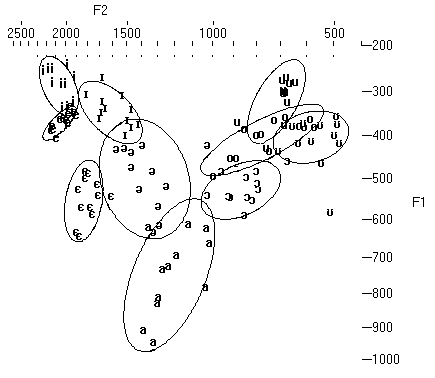
\includegraphics[height=.3\textheight]{figures/OlsonFig1.png}
    \caption{Formant plot of \ili{Ngbugu} vowels (12 tokens each)}
    \label{fig:olson:1}
\end{figure}

Several observations can be made about this plot. First, the \textit{F}\textsubscript{2} of what I have been transcribing as /ɨ/ is generally higher (\char`\~1600 Hz) than the \textit{F}\textsubscript{2} of /ə/ (\char`\~1400 Hz), approaching the front vowels /i/ and /e/. This suggests that /ɨ/ may best be construed as a front vowel. I will transcribe it as /ɪ/ for reasons that will soon become apparent.

Second, the positioning of /ɪ/ and /ʊ/ in the plot generally corresponds to what we expect for high [–ATR] vowels. In \citet{Starwalt2008}’s crosslinguistic study of the acoustics of ATR vowel harmony \is{ATR harmony} systems, she found that the \textit{F}\textsubscript{2} of /ʊ/ is consistently lower than the \textit{F}\textsubscript{2} of /o/ for the \ili{African languages} she studied (although this was not always statistically significant) -- \textit{Kwa} \il{Kwa languages}: \ili{Foodo} [fod] and \ili{Ikposo} [kpo] -- \textit{Bantu} \il{Bantu languages}: \ili{Kinande} [nnb] and \ili{LuBwisi} [tlj] -- \textit{Defoid} \il{Defoid languages}: \ili{Ekiti-Yoruba} [yor]. The positioning of /ʊ/ vis-à-vis /o/ in \figref{fig:olson:1} is consistent with this.

With respect to front vowels, \citeauthor{Starwalt2008} found some variation: for some speakers of \ili{Foodo} (p. 105), \ili{Kinande} (p. 128), and \ili{LuBwisi} (p. 136), the \textit{F}\textsubscript{2} of /ɪ/ is lower than the \textit{F}\textsubscript{2} of /e/. This is consistent with what I found for \ili{Ngbugu}. For the rest of Starwalt’s speakers, the \textit{F}\textsubscript{2} of /ɪ/ was higher than the \textit{F}\textsubscript{2} of /e/.

This acoustic study \is{acoustic analysis} is preliminary. Testing additional subjects would help confirm that our data are indicative of the larger \ili{Ngbugu}-speaking population. \citet{Ladefoged2003} suggests testing a half-dozen speakers of each sex.

\section{Discussion}\label{sec:olson:4}

\subsection{Vowel system symmetry}

If /ɨ/ is reinterpreted as /ɪ/, as proposed in \sectref{sec:olson:3}, the resulting \ili{Ngbugu} vowel system \is{vowel systems} becomes \is{symmetry} symmetric, as shown in \tabref{tab:olson:10}.

\begin{table}
\caption{Reanalyzed \ili{Ngbugu} oral vowel system}
\label{tab:olson:10}
    \begin{tabular}{llll}
    \lsptoprule
                    & front & central   & back\\
    \midrule
        high        & i     &           & u\\
        mid-high    & ɪ     &           & ʊ\\
        mid-low     & e     & ə         & o\\
        low         & ɛ     & a         & (ɔ)\\
    \lspbottomrule
    \end{tabular}
\end{table}

Not only is symmetry what is generally expected for \isi{vowel systems} \citep[59]{Pike1947}, it is also what is found in most languages of the region, as shown in \tabref{tab:olson:11}. The languages of all of the Ubangian \il{Ubangian languages} subgroups except Banda \il{Banda languages} exhibit symmetric \is{symmetry} \isi{vowel systems}, as do many of the languages from the nearby Central Sudanic \il{Central Sudanic languages} group \il{Bongo-Bagirmi languages} Bongo-Bagirmi.

\begin{table}
\caption{Vowel systems of sample languages in geographic proximity ("cross" = cross-height harmony)}
\label{tab:olson:11}
    \begin{tabular}{lllll}
    \lsptoprule
        sample lg & group & oral vowels & VH & source\\
    \midrule
        \ili{Gbeya} & Gbaya \il{Gbaya languages} & /i e ɛ a ɔ o u/ & mid & \citep{Samarin1966}\\
        \ili{Sango} & Ngbandi \il{Ngbandi languages} & /i e ɛ a ɔ o u/ & mid & \citep{Samarin2000}\\
        \ili{Ngbaka Ma'bo} & Sere-Ngb.-Mba \il{Sere-Ngbaka-Mba languages} & /i e ɛ a ɔ o u/ & mid & \citep{Thomas1963}\\
        \ili{Zande} & Zande \il{Zande languages} & /i ɪ ɛ ə a ɔ ʊ u/ & cross & \citep{Boyd1997}\\
        \ili{Nzakara} & Zande \il{Zande languages} & /i ɪ ɛ a ɔ ʊ u/ & cross & \citep{Landi2005}\\
        \ili{Bagiro} & Bongo-Bagirmi \il{Bongo-Bagirmi languages} & /i e ɛ a ɔ o u/ & mid & \citep{Boyeldieu2000}\\
        \ili{Yulu} & Bongo-Bagirmi \il{Bongo-Bagirmi languages} & /i e ɛ (ə) a ɔ o u/ & none & \citep{Boyeldieu1987}\\
        \ili{Lutos} & Bongo-Bagirmi \il{Bongo-Bagirmi languages} & /i e ɛ (ə) a ɔ o u/ & none & \citep{Olson2013}\\
    \lspbottomrule
    \end{tabular}
\end{table}

In fact, the reanalyzed \ili{Ngbugu} vowel system \is{vowel systems} is similar to the set of \ili{Proto-Banda} monophthongs reconstructed by \citeauthor{BoyeldieuCloarec-Heiss2001}, which are shown in \tabref{tab:olson:12}. The differences are (1) the presence of a high central vowel *ɨ, and (2) the absence of the front vowels *ɪ and *ɛ.

\begin{table}
\caption{\ili{Proto-Banda} vowel system \citep{BoyeldieuCloarec-Heiss2001}}
\label{tab:olson:12}
    \begin{tabular}{llll}
    \lsptoprule
                    & front & central   & back\\
    \midrule
        high        & *i    & *ɨ        & *u\\
        mid-high    &       &           & *ʊ\\
        mid-low     & *e    & *ə        & *o\\
        low         &       & *a        & *ɔ\\
    \lspbottomrule
    \end{tabular}
\end{table}

It is not surprising that Boyeldieu and Cloarec-Heiss posited the proto phoneme *ɨ. At the time of their study, it was thought that all \ili{Banda languages} had a high central vowel. The finding that \ili{Ngbugu} has extant /ɪ/ instead opens up the option of positing the proto phoneme *ɪ (rather than *ɨ) with a corresponding \isi{sound change} *ɪ > ɨ to account for the presence of /ɨ/ in the other Banda \il{Banda languages} varieties (subject to confirmation via the comparative method). This also leads to a more typologically \is{typology} common proto vowel system.

As for the absence of *ɛ, \citeauthor{BoyeldieuCloarec-Heiss2001} posit instead the proto diphthong *ia (pp. 198--199). In their analysis, occurrences of [iɛ] in \ili{Ngbugu} following labial, alveolar, and velar consonants are combined with occurrences of [ia] in \ili{Ngbugu} following palatal consonants in order to reconstruct the proto \isi{diphthong}. The corresponding \ili{Linda} forms are [eya] following labials, [ia] following alveolars and velars, and [a] following palatals. Given their data, an equally valid reconstructed form would be *iɛ. Absent from their \isi{correspondence sets} are occurrences of [ɛ].\footnote{There are some residual items in \citeauthor{BoyeldieuCloarec-Heiss2001}'s data: [iɛ] and [ia] contrast in [gia] ‘tourner la pâte’ vs. [giɛ̀] ‘animal, viande’; and [ɛ] and [iɛ] contrast in [ŋgàɛ̀] \char`\~ \space [ŋgɛ̀] ‘canne à sucre’ vs. [ŋgìɛ́] ‘noyau de la noix de palme’ (pp. 192--193).}

If we examine cases of [ɛ], we see that \ili{Ngbugu} [ɛ] corresponds with \ili{Linda} [ja] \citep{Moñino1988} in word-intitial position, as shown in \tabref{tab:olson:13}.

\begin{table}
\caption{Correspondences between \ili{Ngbugu} [ɛ] and \ili{Linda} [ja]}
\label{tab:olson:13}
    \begin{tabular}{lll}
    \lsptoprule
        \ili{Ngbugu} & \ili{Linda} & gloss\\
    \midrule
        ɛ̄.bʁò       & jā.bù.rù  & goat\\
        ɛ̄.vʁó       & jā.vó.ró & dog\\
        ɛ̄.ʃē        & jā.ʃē    & woman\\
    \lspbottomrule
 \end{tabular}
\end{table}

I was not able to identify \isi{cognates} in \ili{Linda} that correspond to the \ili{Ngbugu} words in which [ɛ] is word-medial or word-final. Hence, more research is necessary. That being said, the distinction between the two \isi{correspondence sets} (\ili{Ngbugu} iɛ\char`\~ia vs. \ili{Linda} ia\char`\~eja and \ili{Ngbugu} ɛ vs. \ili{Linda} ja) leads me to propose two proto phonemes, *iɛ and *ɛ, with a possible merger *iɛ, *ɛ > ja in \ili{Linda}. The choice of *ɛ leads to the \ili{Proto-Banda} system in \tabref{tab:olson:14} that is not only typologically \is{typology} more common but is also nearly identical to the extant \ili{Ngbugu} one.

\begin{table}
\caption{Reanalysed \ili{Proto-Banda} vowel system}
\label{tab:olson:14}
 \begin{tabular}{llll}
    \lsptoprule
                    & front & central   & back\\
    \midrule
        high        & *i    &           & *u\\
        mid-high    & *ɪ    &           & *ʊ\\
        mid-low     & *e    & *ə        & *o\\
        low         & *ɛ    & *a        & *ɔ\\
    \lspbottomrule
    \end{tabular}
\end{table}

One mystery of the Banda \il{Banda languages} group has been its unusual inventory of vowels (cf. \tabref{tab:olson:1}). The revised symmetric \ili{Ngbugu} vowel system \is{vowel systems} -- and the comparable \ili{Proto-Banda} system proposed here -- are much more in line with those found in the surrounding languages. Of particular comparative interest are the \isi{vowel systems} of \ili{Nzakara} and \ili{Zande}, since \ili{Nzakara} is the immediate neighbor of \ili{Ngbugu} to the northeast. \ili{Ngbugu}, \ili{Nzakara}, and \ili{Zande} all have identical inventories of \textit{phonetic} vowels: [i ɪ e ɛ ə a ɔ o ʊ u]. These similarities allow for the straightforward comparison of vowels between groups, something that was very difficult given our previous understanding of the \isi{vowel systems} in the Banda \il{Banda languages} group. This makes it more believable that the Banda \il{Banda languages} group could be related to other language groups in the vicinity.

\subsection{\isi{Vowel harmony}}

\citeauthor{BoyeldieuCloarec-Heiss2001} suggest that there are traces of a \ili{Proto-Banda} \isi{ATR harmony} system in extant \ili{Linda} (p. 189), and to a lesser degree in extant \ili{Ngbugu} (pp. 196–197, 202). The existence in the current-day \ili{Ngbugu} vowel system of contrasts between [+ATR] and [–ATR] vowels lends credence to the hypothesis of this earlier \isi{ATR harmony} system.

Indeed, the revised \ili{Ngbugu} vowel inventory bears a remarkable resemblance to inventories that exhibit \isi{ATR harmony}. It is the same inventory as the 10-vowel systems that exhibit the “most straightforward” cases of \isi{ATR harmony} in Africa, where the vowels are divided into two groups: the [+ATR] vowels /i e ə o u/ and the [–ATR] vowels /ɪ ɛ a ɔ ʊ/ \citep[499]{Casali2008}.

Yet, it is relatively clear that the current \ili{Ngbugu} system does not exhibit \isi{vowel harmony}, for two reasons. First, there are many cases in \ili{Ngbugu} of monomorphemic words containing both [+ATR] and [–ATR] vowels, shown in \tabref{tab:olson:15}.

\begin{table}
\caption{Monomorphemic words with both [+ATR] and [–ATR] vowels}
\label{tab:olson:15}
    \begin{tabular}{ll}
    \lsptoprule
        lexical item & gloss\\
    \midrule
        kó.lí.ŋɡʁʊ̄ & millipede\\
        ʃé.ʃɛ̄ & bifurcation\\
        ŋɡèɛ́ & central vein of the palm leaf\\
        ŋɡʊ́.lɛ̀.ʃò & earthworm\\
        kʊ́ɛ́.ló & bitter plant\\
        ŋɡʊ́.wò & smoke\\
        zō.ŋɡʊ̄ & rainy season\\
        à.ɡʁʊ́.mè & midnight\\
        húɛ̄ & sweat\\
        míɛ̄ & twin\\
        tʃá.nə́ & hand\\
        là.fó & standing\\
        mé.ʁà & swell\\
        ā.lū & heavy\\
        à.ɲī & mother\\
    \lspbottomrule
    \end{tabular}
\end{table}

Second, to my knowledge there are no cases of [+ATR] \char`\~ \space [–ATR] alternations in \ili{Ngbugu} roots or affixes \citep[500]{Casali2008}.

The absence of \isi{vowel harmony} in \ili{Ngbugu} is somewhat surprising given the preponderance of harmony systems elsewhere in the region (cf. \tabref{tab:olson:11}). Systems which exhibit harmony between the two sets of mid vowels /e, o/ and /ɛ, ɔ/ (labeled “mid” in \tabref{tab:olson:11}, VH column) are found in the Gbaya \il{Gbaya languages} group (e.g. \ili{Gbeya}), in Sere-Ngbaka-Mba \il{Sere-Ngbaka-Mba languages} (e.g. \ili{Ngbaka-Ma’bo}), and to some degree in the Central Sudanic \il{Central Sudanic languages} group Bongo-Bagirmi \il{Bongo-Bagirmi languages} (e.g. \ili{Bagiro}, which is immediately to the west of the \ili{Ngbugu} region). The \isi{lingua franca} \ili{Sango} from the Ngbandi \il{Ngbandi languages} group also exhibits harmony of this type, but it has exceptions.\footnote{In discussing the simplification of \ili{Sango} vis-à-vis the Ngbandi \il{Ngbandi languages} group, \citet[313]{Samarin2000} states, “Co-occurrence of vowels has been simplified by \isi{vowel harmony}: i.e., mid vowels in a single word are either tense or lax, not both.”}

\isi{Cross-height harmony systems} in which both high and mid vowels undergo \isi{ATR harmony} on a surface phonetic level (labeled “cross” in \tabref{tab:olson:11}, VH column) are found in both \ili{Nzakara} and \ili{Zande}. In these languages, high, mid, and low vowels all undergo \isi{ATR harmony}. For both languages, the mid vowels show harmony only at the surface phonetic level, i.e. [e] and [o] are allophones of /ɛ/ and /ɔ/, respectively. In addition, for \ili{Nzakara} the [a] \char`\~ \space [ə] alternation is also surface phonetic.

The presence of \isi{ATR harmony} in \ili{Nzakara} and \ili{Zande}, the identical inventories of phonetic vowels between \ili{Ngbugu}, \ili{Nzakara}, and \ili{Zande}, and the traces of \isi{ATR harmony} identified by Boyeldieu and Cloarec Heiss for \ili{Linda} and \ili{Ngbugu} -- all these factors lead to the hypothesis that \ili{Proto-Banda} exhibited \isi{ATR harmony}. This harmony system was either inherited or borrowed, and then it was subsequently lost.

What could have led to the loss of \isi{ATR harmony} in \ili{Proto-Banda}? There are at least a couple of factors to consider. First, in a crosslinguistic survey, \citet{RolleEtAl2017} observe that \isi{ATR harmony} and \isi{interior vowels} (e.g. [ɨ], [ə]) appear to be in an antagonistic relationship, and that the presence of both in a given vowel system \is{vowel systems} is dispreferred. Perhaps \ili{Proto-Banda} had both \isi{ATR harmony} and the phoneme /ə/ at some point in its history, and the \isi{ATR harmony} was subsequently lost due to pressure from the interior vowel.

Second, both \citet{Samarin1982} and \citet{Cloarec-Heiss1995} quote \citet[205--206]{Brunache1894} who provides evidence for the existence of a Banda \il{Banda languages} \isi{lingua franca} in the region in the late 19th century. If this is true, the loss of \isi{ATR harmony} may have been a type of simplification of the language structure that is often associated with pidgins \is{pidgin} and \is{lingua franca} lingua francas.

Either of these possibilities -- internal systemic pressure or L2 simplification -- could have contributed a certain instability to the phonological system, leading to the loss of the \isi{ATR harmony}, as well as other eventual structural changes.

\section{Conclusion}\label{sec:olson:5}

In summary, extant \ili{Ngbugu} has a symmetric \is{symmetry} vowel system \is{vowel systems} (including one \is{interior vowels}interior vowel) that resembles \isi{vowel systems} of the other groups in the region, except for the absence of \isi{vowel harmony}. The extant ATR contrasts in \ili{Ngbugu} lend support to Boyeldieu and Cloarec-Heiss’s reconstructed \ili{Proto-Banda} vowel system \is{vowel systems} containing ATR contrasts. The traces of a \isi{vowel harmony} system in \ili{Linda} and \ili{Ngbugu}, combined with the similarity of \ili{Ngbugu}’s surface phonetic vowel inventory to that of nearby languages that exhibit \isi{vowel harmony} (particularly \ili{Nzakara}) support the hypothesis that \ili{Proto-Banda} may have had \isi{vowel harmony} at some point in its history.

\section*{Acknowledgements}

I wish to thank Tychique Longbo, Jessé-Joël Adoumacho, and Guy-Florent Matchi for their collaboration and friendship, Connie Kutsch Lojenga for assistance with the methodology (and in particular being the first to identify /ʊ/), Pascal Boyeldieu, Mike Cahill, Bill Samarin, Coleen Starwalt, and participants at ACAL 49 for helpful comments (all errors are my own), and the SIL Central African Republic Service Group for funding.

\printbibliography[heading=subbibliography,notkeyword=this]

\end{document}
